\documentclass[11pt,a4paper]{article}
\usepackage[margin=22mm]{geometry}
\usepackage[T1]{fontenc}
\usepackage{lmodern,booktabs,tabularx,longtable,array,graphicx,float,xcolor,listings,microtype,fancyhdr}
\usepackage[hyphens]{url}
\usepackage[colorlinks=true,linkcolor=black,urlcolor=blue]{hyperref}
\definecolor{ink}{HTML}{17324D}
\definecolor{light}{HTML}{F3F5F7}
\setlength{\parindent}{0pt}
\setlength{\parskip}{5pt}
\setlength{\emergencystretch}{3em}
\renewcommand{\arraystretch}{1.18}
\pagestyle{fancy}\fancyhf{}\lhead{\small A17 / PlantUML}\rhead{\small 23CSE455 Design Patterns}\cfoot{\thepage}
\setlength{\headheight}{14pt}
\lstset{basicstyle=\ttfamily\footnotesize,breaklines=true,columns=fullflexible,keepspaces=true,backgroundcolor=\color{light},frame=single,rulecolor=\color{light},xleftmargin=4pt,xrightmargin=4pt,showstringspaces=false}
\begin{document}
\begin{titlepage}
\vspace*{10mm}
{\large 23CSE455 Design Patterns\par}
\vspace{16mm}
{\Huge\bfseries Case Study Report\par}
\vspace{9mm}
{\LARGE\color{ink} Design Pattern Analysis and Evolution in the PlantUML Diagram Generation System\par}
\vspace{12mm}
{\large Team A17\par}
\vspace{5mm}
\begin{tabularx}{\linewidth}{@{}lXl@{}}\toprule
Roll number & Student name & Batch\\\midrule
AM.SC.U4CSE23064 & Sathvik Pasuvula & CSE A\\
AM.SC.U4CSE23142 & P Sai Satvik Chowdary & CSE A\\\bottomrule
\end{tabularx}
\par\vspace{7mm}\noindent
\textbf{Application:}\hspace{0.6em}PlantUML, class-diagram family\\
\textbf{Selected baseline:}\hspace{0.6em}v1.2026.8\\
\textbf{Date:}\hspace{0.6em}2026-10-11\\
\textbf{Submission repository:}\hspace{0.6em}\href{https://github.com/aswathymohan-amrita/23CSE455_DP_CaseStudy}{23CSE455\_DP\_CaseStudy}
\vfill
\textbf{Scope of this submission}\par
Five source-verified GoF collaborations, three implemented changes, and equivalent
four-language examples. Source snapshots, patches, tests, raw timings and datasets
accompany this report. Human review, contribution confirmation, faculty approval
and repository merge are explicitly separated from automated verification.
\end{titlepage}
\tableofcontents\newpage
\section{Application and architecture}
PlantUML converts a textual description into a diagram. This study follows class
declarations and an association through command recognition, model construction,
layout, styling and image export. Its purpose is to test pattern claims against
working source, then observe what actually changes when requirements evolve.

\textbf{Original source.} The official baseline is
\href{https://github.com/plantuml/plantuml/tree/v1.2026.8}{PlantUML v1.2026.8}, accessed
2026-10-11. The peeled commit is
\path{149874a1bb2b64c42889d7178cb89f6647ac14bc}. The annotated tag object is
\path{b531f7b00ebf733d9079a7b0a0180c64ded21ef0}; these hashes are not interchangeable.
The inspected source distribution uses GPL v3-or-later notices. Upstream license
files accompany the copied source. Faculty approval was not supplied in this interaction.

\textbf{Environment.} The runs used macOS 27.0.1 on arm64, OpenJDK 25.0.2,
Gradle 9.3.1 and Graphviz 16.1.0. Production Java was compiled with release 11.
The snippets used Python 3.14.2, Node.js 22.19.0 and Apple clang 21.0.0 with C++17.
There is no database in the inspected path. The baseline dependency catalog pins
JUnit 6.1.3, ELK 0.12.0, TeaVM 0.14.1, JLaTeXMath 1.0.7 and OpenPDF 3.0.5.
The backend-specific dependencies are not all needed by the small class example.

\textbf{Scope.} The inventory investigates the five pattern types named in the
brief: Command, Factory Method, Strategy, Composite and Adapter. It covers
class commands, their receiver objects, layout backend selection, class-header
text blocks and the VizJs output bridge. It is a representative collaboration
study, not a census of all PlantUML commands or every TextBlock implementation.
Sequence/activity families, web-server internals, browser execution and optional
VizJs runtime installation are excluded from the integration experiment.
All mapped participant classes are recorded in \path{data/patterns.csv}; the
local source subset preserves upstream paths under \path{data/code/}.

\subsection{Architecture and a concrete input trace}
\begin{figure}[H]\centering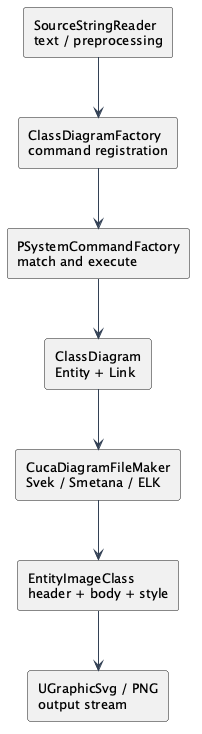
\includegraphics[width=\linewidth,height=103mm,keepaspectratio]{Part1/diagrams/architecture.png}\caption{Class-diagram processing path. Each box identifies a responsibility, not a separate process.}\end{figure}
\begin{lstlisting}
@startuml
class Order
class Customer
Order --> Customer
@enduml
\end{lstlisting}
\begin{enumerate}
\item \texttt{SourceStringReader} preprocesses the text into diagram blocks.
\texttt{ClassDiagramFactory} creates a \texttt{ClassDiagram} and registers commands.
\item \texttt{PSystemCommandFactory.getCandidate} tests registered commands against
the current line. Its execution loop calls \texttt{AbstractDiagram.executeCommand},
which wraps execution in \texttt{ProtectedCommand} and delegates to the command.
\item \texttt{CommandCreateClass.executeArg} resolves the identifier in the diagram
context, creates or updates an \texttt{Entity}, then attaches display and style data.
\texttt{CommandLinkClass.executeArg} resolves the endpoints, constructs a
\texttt{Link}, and adds it to the diagram. The checked model has two nodes and one link.
\item \texttt{CucaDiagram.getTextBlock} selects a layout backend. The normal desktop
path can use Svek with Graphviz; the repeatable integration fixture adds
\texttt{!pragma layout smetana} to select in-process Java layout.
\item \texttt{EntityImageClass} combines header and body blocks. Style signatures
merge defaults and stereotype/style rules; explicit entity colors can override
the relevant values. This is the point extended by the review palette.
\item \path{SourceStringReader.outputImage} calls the diagram's export method.
\path{UgDiagram.exportDiagram} obtains a \texttt{TextBlockExporter}, which creates
the format-specific drawing context and writes to the output stream. For SVG,
group attributes reach \texttt{PortableSvgDocument}; PNG uses its raster drawing path.
\end{enumerate}
\begin{figure}[H]\centering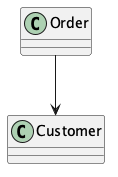
\includegraphics[width=\linewidth,height=42mm,keepaspectratio]{Part1/evidence/baseline.png}\caption{Baseline input rendered through the default desktop layout path with Graphviz installed.}\end{figure}
\textbf{Run results.} Both complete source trees produced a JAR. Running
\texttt{GPL\_ONLY=1 bash gradlew jar test -Pfast --console=plain} on each tree
reported 3,189 tests: 3,177 passed, 2 failed, 10 skipped. The JUnit XML and
generated HTML report count 3,191 entries (3,177 passed, 2 failed, 12 skipped),
including two additional skipped entries. Both trees show the same discrepancy;
these totals are identified by evidence source rather than merged. Both failures are in
\texttt{PicowebTest}: \texttt{get\_png\_bad\_graphviz} and
\texttt{get\_png\_svg\_graphviz}, each expecting HTTP 200 but receiving 503.
The same failures occur before and after the changes. Their cause is not resolved
here; the complete suite is not described as passing. The focused baseline checks
passed 3/3 and the final full-JAR integration checks passed 20/20. Commands and raw
logs are linked from \path{README.md}.

\section{Part 1: Pattern discovery}
\subsection{Method and counting rules}
Candidate discovery began with source searches, but a class name was not accepted
as proof. Each confirmed record requires an intent, a shared contract, identifiable
participants and a call or ownership relationship that explains the behavior.
The source mapping is commit-specific. Runtime tests establish the selected input
path; source-only claims for optional backends are explicitly marked.

One record represents one collaboration. Multiple concrete commands do not become
multiple Command instances. The baseline has five distinct pattern types and five
instances. It maps 13 concrete classes in the varying GoF roles and 30 unique
participant symbols including shared abstractions, clients and receiver objects.
The concrete count includes concrete products for Factory Method and the selected
composites/leaf for Composite; it excludes fixed contexts and assembly helpers.
These are counts of mapped representatives, not of every implementation in PlantUML.

\begin{tabularx}{\linewidth}{@{}lXrr@{}}\toprule
Pattern & Collaboration & Instances & Concrete\\\midrule
Command & Class diagram command dispatch & 1 & 3\\
Factory Method & Class diagram product creation & 1 & 2\\
Strategy & Class diagram layout backend selection & 1 & 4\\
Composite & Class header text-block composition & 1 & 3\\
Adapter & VizJs output-stream bridge & 1 & 1\\\bottomrule
\end{tabularx}

Two observations are rejected: Entity/Link membership alone does not prove
Composite, and same-interface forwarding by UGraphicDelegator does not prove
Adapter. One older candidate, text-block PlacementStrategy, remains uncertain
within this input trace because its context was not fully mapped. It is excluded
from confirmed counts. Template Method, Builder and graphics decorators are
supporting idioms outside this five-type inventory; no absence claim is made.

\textbf{Reading the mapping tables.} All symbols below are actual source symbols.
Except \texttt{net.atmp.CucaDiagram}, they use the prefix
\texttt{net.sourceforge.plantuml.} The source column omits
\path{data/code/src/main/java/net/sourceforge/plantuml/}; full paths and complete
line ranges are in the CSV. A range spans the participant declaration and body;
the named methods identify the relevant behavior.

\clearpage
\subsection{Command: Class diagram command dispatch}
\textbf{Category and origin.} GoF behavioral pattern; baseline application code.

\textbf{Intent.} Encapsulate recognized source instructions as interchangeable executable objects, separating command selection from model mutation.

\begin{longtable}{@{}p{.22\linewidth}p{.73\linewidth}@{}}\toprule Role & Actual symbol, methods and source\\\midrule\endhead
Command & \path{command.Command}\newline isValid; execute\newline {\footnotesize\path{command/Command.java}:42--58}\\
Shared command implementation & \path{command.SingleLineCommand2}\newline execute; executeArg\newline {\footnotesize\path{command/SingleLineCommand2.java}:51--193}\\
ConcreteCommand & \path{classdiagram.command.CommandCreateClass}\newline getRegexConcat; executeArg\newline {\footnotesize\path{classdiagram/command/CommandCreateClass.java}:71--247}\\
ConcreteCommand & \path{classdiagram.command.CommandLinkClass}\newline executeArg; addLink\newline {\footnotesize\path{classdiagram/command/CommandLinkClass.java}:73--553}\\
ConcreteCommand & \path{command.CommandPragma}\newline executeArg\newline {\footnotesize\path{command/CommandPragma.java}:52--139}\\
Invoker/selector & \path{command.PSystemCommandFactory}\newline getCandidate; executeFewLines\newline {\footnotesize\path{command/PSystemCommandFactory.java}:61--309}\\
Execution bridge & \path{core.AbstractDiagram}\newline executeCommand\newline {\footnotesize\path{core/AbstractDiagram.java}:67--273}\\
Client/registration & \path{classdiagram.ClassDiagramFactory}\newline initCommandsList\newline {\footnotesize\path{classdiagram/ClassDiagramFactory.java}:88--173}\\
Receiver & \path{classdiagram.ClassDiagram}\newline inherited reallyCreateLeaf; addLink\newline {\footnotesize\path{classdiagram/ClassDiagram.java}:49--101}\\
Receiver base & \path{objectdiagram.AbstractClassOrObjectDiagram}\newline class diagram shared model\newline {\footnotesize\path{objectdiagram/AbstractClassOrObjectDiagram.java}:60--365}\\
Model element & \path{abel.Entity}\newline setColors; setStereotype\newline {\footnotesize\path{abel/Entity.java}:89--775}\\
Model relationship & \path{abel.Link}\newline constructor\newline {\footnotesize\path{abel/Link.java}:65--580}\\
\bottomrule\end{longtable}
\textbf{Evidence and interpretation.} PSystemCommandFactory.getCandidate selects a Command using isValid; executeFewLines delegates through AbstractDiagram.executeCommand. CommandCreateClass.executeArg creates or updates an Entity; CommandLinkClass.executeArg creates a Link and adds it to the receiver. CommandPragma handles the layout directive in the traced input. No undo/history support is claimed.

\noindent\textit{net/sourceforge/plantuml/command/PSystemCommandFactory.java, lines 230--239}
\begin{lstlisting}
		for (Command cmd : cmds) {
			final CommandControl result = safeIsValid(cmd, single);
			if (result == CommandControl.OK) {
				it.next();
				return new Step(cmd, single);
			}
			if (result == CommandControl.OK_PARTIAL) {
				final IteratorCounter2 cloned = it.cloneMe();
				final BlocLines lines = isMultilineCommandOk(cloned, cmd);
				if (lines == null)
\end{lstlisting}
\begin{figure}[H]\centering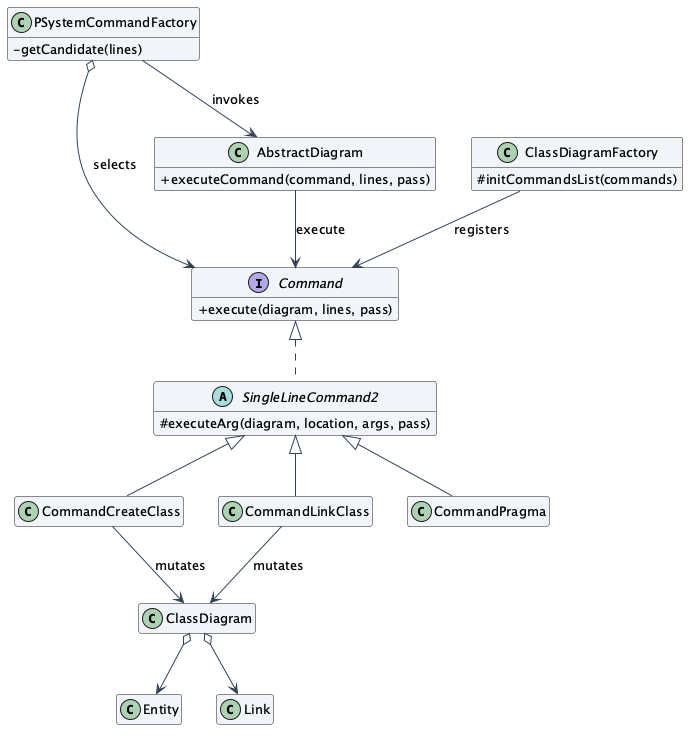
\includegraphics[width=\linewidth,height=90mm,keepaspectratio]{Part1/diagrams/command.png}\caption{Class diagram command dispatch. Abbreviated names correspond to the mapping above.}\end{figure}
Adding syntax changes the relevant command rather than the parser loop. The receiver still exposes a substantial mutable model API, so Command does not eliminate parser-to-model coupling. The chosen commands are stateless handlers; there is no claim that they support undo or replay history.

\textbf{Verification.} Confirmed by source inspection in this automated run. Human reviewer pending. Editable UML and PNG/SVG outputs: \path{Part1/diagrams/command.puml}. Detailed evidence: \path{Part1/evidence/command.md}.

\clearpage
\subsection{Factory Method: Class diagram product creation}
\textbf{Category and origin.} GoF creational pattern; baseline application code.

\textbf{Intent.} Let a specialized parser factory choose the diagram product while the superclass retains the parsing lifecycle.

\begin{longtable}{@{}p{.22\linewidth}p{.73\linewidth}@{}}\toprule Role & Actual symbol, methods and source\\\midrule\endhead
Creator & \path{command.PSystemCommandFactory}\newline createSystem; createEmptyDiagram\newline {\footnotesize\path{command/PSystemCommandFactory.java}:61--309}\\
ConcreteCreator & \path{classdiagram.ClassDiagramFactory}\newline createEmptyDiagram\newline {\footnotesize\path{classdiagram/ClassDiagramFactory.java}:88--173}\\
Product & \path{core.AbstractDiagram}\newline executeCommand; exportDiagram contract\newline {\footnotesize\path{core/AbstractDiagram.java}:67--273}\\
ConcreteProduct & \path{classdiagram.ClassDiagram}\newline constructor\newline {\footnotesize\path{classdiagram/ClassDiagram.java}:49--101}\\
\bottomrule\end{longtable}
\textbf{Evidence and interpretation.} PSystemCommandFactory.createSystem calls the abstract createEmptyDiagram hook. ClassDiagramFactory overrides it with a covariant ClassDiagram return and constructs that product. This is a virtual creation hook used by superclass code, not merely a helper named factory.

\noindent\textit{net/sourceforge/plantuml/classdiagram/ClassDiagramFactory.java, lines 94--99}
\begin{lstlisting}
	@Override
	public ClassDiagram createEmptyDiagram(PathSystem pathSystem, UmlSource source, Previous previous,
			PreprocessingArtifact preprocessing) {
		return new ClassDiagram(source, previous, preprocessing);
	}

\end{lstlisting}
\begin{figure}[H]\centering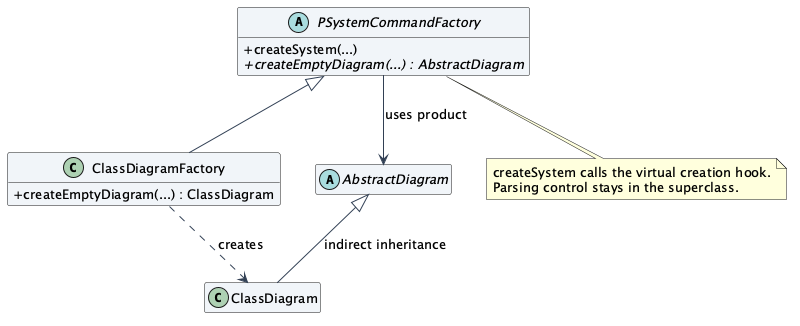
\includegraphics[width=\linewidth,height=65mm,keepaspectratio]{Part1/diagrams/factory.png}\caption{Class diagram product creation. Abbreviated names correspond to the mapping above.}\end{figure}
The factory method preserves a common parse lifecycle across diagram families. It relies on inheritance at the creation boundary. A static helper returning a new ClassDiagram would not have the same subclass-controlled creation intent.

\textbf{Verification.} Confirmed by source inspection in this automated run. Human reviewer pending. Editable UML and PNG/SVG outputs: \path{Part1/diagrams/factory.puml}. Detailed evidence: \path{Part1/evidence/factory.md}.

\clearpage
\subsection{Strategy: Class diagram layout backend selection}
\textbf{Category and origin.} GoF behavioral pattern; baseline application code.

\textbf{Intent.} Select a layout algorithm without forcing the caller to know each backend's graph processing steps.

\begin{longtable}{@{}p{.22\linewidth}p{.73\linewidth}@{}}\toprule Role & Actual symbol, methods and source\\\midrule\endhead
Context & \path{net.atmp.CucaDiagram}\newline getTextBlock; dotIsAvailable\newline {\footnotesize\path{src/main/java/net/atmp/CucaDiagram.java}:109--959}\\
Strategy & \path{svek.CucaDiagramFileMaker}\newline getTextBlock\newline {\footnotesize\path{svek/CucaDiagramFileMaker.java}:46--71}\\
ConcreteStrategy & \path{svek.CucaDiagramFileMakerSvek}\newline getTextBlock\newline {\footnotesize\path{svek/CucaDiagramFileMakerSvek.java}:52--116}\\
ConcreteStrategy & \path{sdot.CucaDiagramFileMakerSmetana}\newline getTextBlock\newline {\footnotesize\path{sdot/CucaDiagramFileMakerSmetana.java}:116--925}\\
ConcreteStrategy & \path{elk.CucaDiagramFileMakerElk}\newline getTextBlock\newline {\footnotesize\path{elk/CucaDiagramFileMakerElk.java}:138--501}\\
ConcreteStrategy & \path{svek.CucaDiagramFileMakerTeaVM}\newline getTextBlock\newline {\footnotesize\path{svek/CucaDiagramFileMakerTeaVM.java}:56--148}\\
\bottomrule\end{longtable}
\textbf{Evidence and interpretation.} CucaDiagram.getTextBlock selects a CucaDiagramFileMaker based on TeaVM, ELK, Smetana and Graphviz availability, then delegates to getTextBlock with the same arguments. Svek uses the external dot pipeline; Smetana performs layout in Java. ELK and TeaVM branches are source-verified but not exercised by the A17 tests.

\noindent\textit{net/atmp/CucaDiagram.java, lines 478--485}
\begin{lstlisting}
		else if (this.isUseElk())
			maker = new CucaDiagramFileMakerElk(this);
		else if (this.isUseSmetana() || this.dotIsAvailable() == false)
			maker = new CucaDiagramFileMakerSmetana(this);
		else
			maker = new CucaDiagramFileMakerSvek(this);

		return maker.getTextBlock(getDotStrings(), fileFormatOption);
\end{lstlisting}
\begin{figure}[H]\centering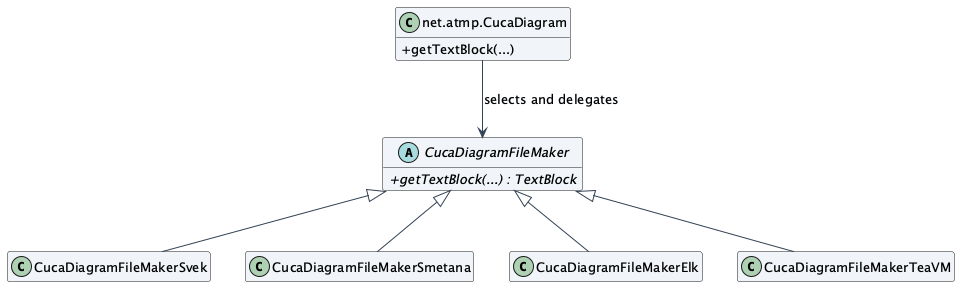
\includegraphics[width=\linewidth,height=65mm,keepaspectratio]{Part1/diagrams/strategy.png}\caption{Class diagram layout backend selection. Abbreviated names correspond to the mapping above.}\end{figure}
The selected object is local to getTextBlock; Strategy does not require a long-lived field. Selection remains a conditional in the context, so registering a completely new backend still requires editing that selection. Existing backends share the TextBlock result contract.

\textbf{Verification.} Confirmed by source inspection in this automated run. Human reviewer pending. Editable UML and PNG/SVG outputs: \path{Part1/diagrams/strategy.puml}. Detailed evidence: \path{Part1/evidence/strategy.md}.

\clearpage
\subsection{Composite: Class header text-block composition}
\textbf{Category and origin.} GoF structural pattern; baseline application code.

\textbf{Intent.} Treat a single drawable and an aggregate of drawables through the same measurement and drawing interface.

\begin{longtable}{@{}p{.22\linewidth}p{.73\linewidth}@{}}\toprule Role & Actual symbol, methods and source\\\midrule\endhead
Component & \path{klimt.shape.TextBlock}\newline calculateDimension; inherited drawU\newline {\footnotesize\path{klimt/shape/TextBlock.java}:47--67}\\
Composite base & \path{klimt.shape.TextBlockMemoized}\newline calculateDimension; calculateDimensionSlow\newline {\footnotesize\path{klimt/shape/TextBlockMemoized.java}:50--72}\\
Composite & \path{klimt.shape.TextBlockHorizontal}\newline calculateDimensionSlow; drawU\newline {\footnotesize\path{klimt/shape/TextBlockHorizontal.java}:48--95}\\
Composite & \path{klimt.shape.TextBlockVertical}\newline calculateDimensionSlow; drawU\newline {\footnotesize\path{klimt/shape/TextBlockVertical.java}:51--134}\\
Representative leaf & \path{klimt.shape.CircledCharacter}\newline calculateDimension; drawU\newline {\footnotesize\path{klimt/shape/CircledCharacter.java}:46--88}\\
Client & \path{svek.image.EntityImageClassHeader}\newline constructor\newline {\footnotesize\path{svek/image/EntityImageClassHeader.java}:74--279}\\
Assembly helper & \path{klimt.shape.TextBlockUtils}\newline mergeLR; mergeTB\newline {\footnotesize\path{klimt/shape/TextBlockUtils.java}:55--183}\\
\bottomrule\end{longtable}
\textbf{Evidence and interpretation.} TextBlockHorizontal and TextBlockVertical hold lists of TextBlock children, recursively measure them, and draw each through the component interface with translated coordinates. CircledCharacter is the inspected leaf. EntityImageClassHeader builds the header from smaller blocks through TextBlockUtils. The entity/link graph itself is not the evidence for Composite.

\noindent\textit{net/sourceforge/plantuml/klimt/shape/TextBlockHorizontal.java, lines 68--77}
\begin{lstlisting}
	@Fast
	public XDimension2D calculateDimensionSlow(StringBounder stringBounder) {
		XDimension2D dim = blocks.get(0).calculateDimension(stringBounder);
		for (int i = 1; i < blocks.size(); i++)
			dim = dim.mergeLR(blocks.get(i).calculateDimension(stringBounder));

		return dim;
	}

	@Override
\end{lstlisting}
\begin{figure}[H]\centering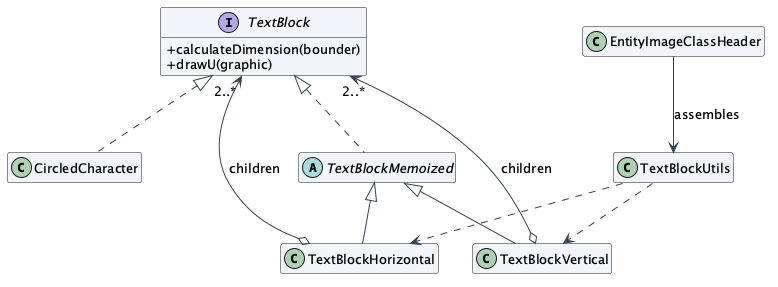
\includegraphics[width=\linewidth,height=65mm,keepaspectratio]{Part1/diagrams/composite.png}\caption{Class header text-block composition. Abbreviated names correspond to the mapping above.}\end{figure}
A client can measure and draw an aggregate through TextBlock, and composites recursively invoke that same contract on their children. The selected leaf is CircledCharacter. Other rich-text leaves and margin wrappers exist; their complete implementation families are not included in the participant count.

\textbf{Verification.} Confirmed by source inspection in this automated run. Human reviewer pending. Editable UML and PNG/SVG outputs: \path{Part1/diagrams/composite.puml}. Detailed evidence: \path{Part1/evidence/composite.md}.

\clearpage
\subsection{Adapter: VizJs output-stream bridge}
\textbf{Category and origin.} GoF structural pattern; baseline application code.

\textbf{Intent.} Expose a string-returning JavaScript layout engine through PlantUML's existing Graphviz output-stream interface.

\begin{longtable}{@{}p{.22\linewidth}p{.73\linewidth}@{}}\toprule Role & Actual symbol, methods and source\\\midrule\endhead
Target & \path{dot.Graphviz}\newline createFile3\newline {\footnotesize\path{dot/Graphviz.java}:41--52}\\
Adapter & \path{vizjs.GraphvizJs}\newline createFile3; submitJob\newline {\footnotesize\path{vizjs/GraphvizJs.java}:52--153}\\
Adaptee facade & \path{vizjs.VizJsEngine}\newline execute\newline {\footnotesize\path{vizjs/VizJsEngine.java}:41--68}\\
Client & \path{svek.DotStringFactory}\newline getSvg; createFile3 call\newline {\footnotesize\path{svek/DotStringFactory.java}:70--654}\\
Adapter selection & \path{dot.GraphvizRuntimeEnvironment}\newline create\newline {\footnotesize\path{dot/GraphvizRuntimeEnvironment.java}:56--238}\\
\bottomrule\end{longtable}
\textbf{Evidence and interpretation.} GraphvizJs implements Graphviz.createFile3(OutputStream). It submits a VizJsEngine.execute(dotString) operation, obtains its SVG String, writes bytes to the requested stream and returns ProcessState. VizJsEngine reflectively calls ch.braincell.viz.VizJS. This incompatible-interface conversion establishes Adapter intent. Optional VizJs execution is not claimed.

\noindent\textit{net/sourceforge/plantuml/vizjs/GraphvizJs.java, lines 88--100}
\begin{lstlisting}
	public GraphvizJs(String dotString) {
		this.dotString = dotString;
	}

	public ProcessState createFile3(OutputStream os) {
		try {
			final String svg = submitJob().get();
			os.write(svg.getBytes());
			return ProcessState.TERMINATED_OK();
		} catch (Exception e) {
			Logme.error(e);
			throw new GraphvizJsRuntimeException(e);
		}
\end{lstlisting}
\begin{figure}[H]\centering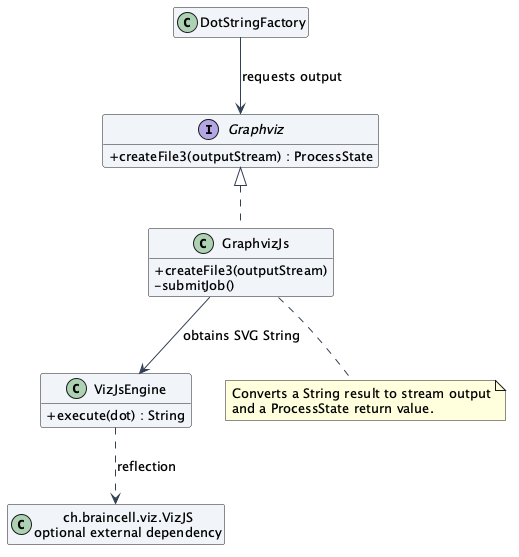
\includegraphics[width=\linewidth,height=65mm,keepaspectratio]{Part1/diagrams/adapter.png}\caption{VizJs output-stream bridge. Abbreviated names correspond to the mapping above.}\end{figure}
The mismatch is concrete: an engine returns a String, while the caller requires stream output and ProcessState. The adapter also manages asynchronous execution. This source evidence confirms the collaboration, but the optional ch.braincell VizJS dependency was not installed or executed.

\textbf{Verification.} Confirmed by source inspection in this automated run. Human reviewer pending. Editable UML and PNG/SVG outputs: \path{Part1/diagrams/adapter.puml}. Detailed evidence: \path{Part1/evidence/adapter.md}.

\clearpage
\section{Part 2: Evolution and refactoring}
The three changes form a small review workflow for class diagrams. Status is stored
once in the model, rendered as a visible label, optionally mapped to a fill policy,
and optionally exposed to SVG consumers. Existing tags and stereotypes can label
classes, but do not provide this constrained property and its dedicated output
contract. The implementation therefore extends existing mechanisms instead of
claiming that annotations, colors or metadata were absent.

\subsection{CH01: Explicit review status on a class declaration}
\textbf{Requirement.} A single-line declaration accepts a final
\texttt{[review=pending]}, \texttt{[review=approved]} or
\texttt{[review=rejected]} option. Matching is case-insensitive. Omitted status
preserves the current value on redeclaration; an explicit status replaces it.
The label appears in the class header. Existing class/link topology is unchanged.
Unknown values must produce a parse error.
\begin{lstlisting}
@startuml
!pragma layout smetana
class Order [review=pending]
class Customer [review=approved]
Order --> Customer
@enduml
\end{lstlisting}
\begin{figure}[H]\centering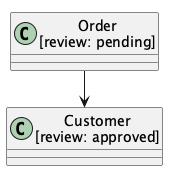
\includegraphics[width=\linewidth,height=52mm,keepaspectratio]{Part2/evidence/CH01/review.png}\caption{CH01: explicit review labels on the two class headers.}\end{figure}
\textbf{Impact.} \texttt{CommandCreateClass.getRegexConcat} recognizes the
suffix and \texttt{executeArg} stores it. \texttt{Entity} gains the property and
accessors. \texttt{EntityImageClassHeader} adds a display line before building the
name TextBlock. No dispatcher replacement or separate diagram subtype is needed.

\textbf{Acceptance evidence.} 11/11 focused checks passed, covering valid states,
unknown-state rejection, model counts, redeclaration, explicit color coexistence
and PNG/SVG output. The production API's setter is intentionally small; syntax
validation occurs in the command. Multiline declaration syntax and text/XMI
exports are not extended. The option can be declared on a separate line before
adding members. This boundary is part of the requirement, not an untested claim
that every serializer supports the new property.

\textbf{Pattern effect.} Command is modified in one concrete handler. Factory
Method, layout Strategy, text-block Composite and VizJs Adapter remain preserved.
The Composite tree receives different text; that does not create a second
Composite collaboration. No unrelated refactoring is claimed for CH01.

\subsection{CH02: Configurable review styling policy}
\textbf{Requirement.} \texttt{!pragma classReviewPalette} accepts
\texttt{default}, \texttt{pastel} or \texttt{mono}. Default retains normal style
resolution. Pastel maps pending to \texttt{\#FFF3CD}, approved to
\texttt{\#D4EDDA} and rejected to \texttt{\#F8D7DA}; mono uses
\texttt{\#EEEEEE} for all reviewed nodes. Explicit class fill wins over the
policy. Unreviewed nodes retain existing styles. The policy changes fill only;
it is not a guarantee of accessibility for arbitrary custom fonts and themes.
\begin{lstlisting}
@startuml
!pragma layout smetana
!pragma classReviewPalette pastel
class Order [review=pending]
class Customer [review=approved]
Order --> Customer
@enduml
\end{lstlisting}
\begin{figure}[H]\centering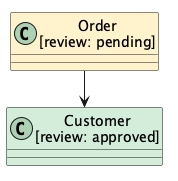
\includegraphics[width=\linewidth,height=52mm,keepaspectratio]{Part2/evidence/CH02/palette.png}\caption{CH02: state-dependent pastel fill. Text labels remain useful when colors are unavailable.}\end{figure}
\textbf{Impact.} \texttt{CommandPragma} validates the option and
\texttt{PragmaKey} records it. \path{EntityImageClass.drawInternal} reads the
existing review property and asks a \texttt{ReviewPalette} for its fill. The nested
\texttt{Pastel} and \texttt{Mono} classes implement the same operation.
The client tests whether an explicit color already exists before applying the policy.

\textbf{Acceptance evidence.} 15/15 cumulative checks passed. Both policy choices,
invalid-value rejection and explicit-color precedence are tested. A failed early
assertion was corrected after observing that the SVG writer abbreviates
\texttt{\#EEEEEE} to \texttt{\#EEE}; the color itself was correct.

\textbf{Pattern effect.} A new Strategy instance, \emph{Review-state fill policy},
is introduced. The original layout Strategy keeps its name and count. Command
is modified to validate the pragma. Other mapped collaborations are preserved.
The small interface makes policy behavior independently replaceable, but the
selector still enumerates policy names. Two classes are a deliberate trade-off
for the course experiment; this is not evidence that every two-color rule needs
a Strategy hierarchy.

\subsection{CH03: Optional SVG metadata and a local refactoring}
\textbf{Requirement.} \texttt{!pragma svgReviewMetadata true} adds
\texttt{data-review-status} to reviewed entity groups. The default and explicit
\texttt{false} omit it. Unreviewed entities do not receive an empty attribute.
Only true/false are accepted. The diagram's visible output is unchanged.
\begin{lstlisting}
@startuml
!pragma layout smetana
!pragma svgReviewMetadata true
class Order [review=pending]
class Customer [review=approved]
Order --> Customer
@enduml
\end{lstlisting}
\begin{figure}[H]\centering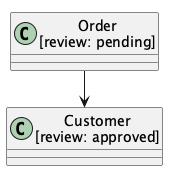
\includegraphics[width=\linewidth,height=52mm,keepaspectratio]{Part2/evidence/CH03/metadata.png}\caption{CH03: the visible diagram is unchanged; additional information is in SVG group attributes.}\end{figure}
\begin{lstlisting}
<g class="entity" ... data-review-status="pending" ...>
  <!-- Order shapes and label -->
</g>
\end{lstlisting}
The fragment above abbreviates unrelated SVG attributes. The complete output
is \path{Part2/evidence/CH03/metadata.svg}.

\textbf{Impact.} The validated pragma is read by \texttt{EntityImageClass}, which
adds a \path{UGroupType.DATA_REVIEW_STATUS} entry. The portable SVG serializer
must explicitly allow that key. The first implementation reached the group but
failed the integration test because the serializer ignored the unfamiliar key.
Extending the allow-list fixed the defect. This shows why tracing only parser and
model code would have missed a real output integration requirement.

\textbf{Refactoring.} \texttt{drawInternal} previously requested the same merged
style separately for shadow, border, background and stroke. A local
\texttt{resolvedStyle} now supplies those values. This is removal of redundant
style lookups, not a pattern replacement. The recorded CH02 and CH03
\texttt{review.svg} outputs are byte-identical with metadata disabled.

\textbf{Acceptance evidence.} 20/20 cumulative checks passed, including enabled,
default-off, explicit-off, missing-status and invalid-value cases. The same 20
checks passed against the JAR produced by the complete modified source build.
All format-specific claims are limited to SVG metadata and the PNG/SVG visible
outputs exercised here. No new file format or sidecar is claimed.
\begin{figure}[H]\centering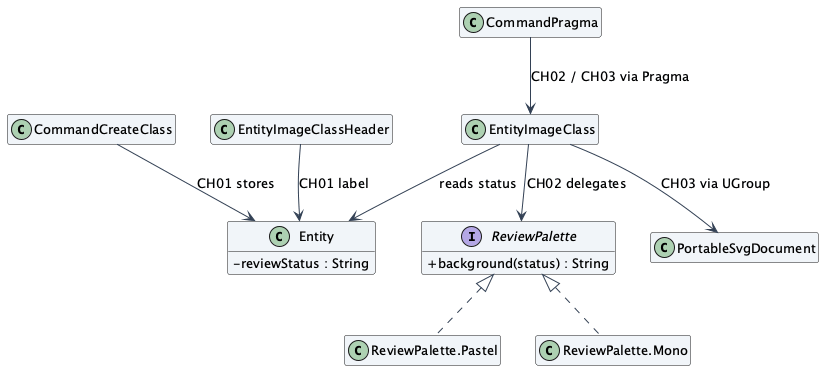
\includegraphics[width=\linewidth,height=78mm,keepaspectratio]{Part2/diagrams/review-policy.png}\caption{Changed responsibilities across parser, model, styling and SVG output.}\end{figure}
\subsection{Snapshots, metrics and pattern effects}
Each change has a separate source commit, cumulative source snapshot, patch and
test log in \path{Part2/changes/Change1}, \path{Change2} and \path{Change3}.
The patches apply consecutively to the recorded baseline. Commit IDs identify
the local experiment; the patch and saved source allow reproduction without
requiring those student commits to be published upstream.
\begin{longtable}{@{}lp{.8\linewidth}@{}}\toprule Snapshot & Exact commit\\\midrule\endhead
Baseline & \path{149874a1bb2b64c42889d7178cb89f6647ac14bc}\\
CH01 & \path{8e9f313b8f589012115d631df4aad2a369a22f53}\\
CH02 & \path{0d170a89f61fc811f729f236a28634c697f985a6}\\
CH03 & \path{dd5c91b457c13fb1a20ae51a62fa73c3b8485847}\\
\bottomrule\end{longtable}
\begin{tabularx}{\linewidth}{@{}lrrrrX@{}}\toprule
Snapshot & LOC & Max CC & Types & Instances & Focused tests\\\midrule
Baseline & 1314 & 20 & 5 & 5 & 3/3\\
CH01 & 1329 & 20 & 5 & 5 & 11/11\\
CH02 & 1366 & 20 & 5 & 6 & 15/15\\
CH03 & 1376 & 20 & 5 & 6 & 20/20\\
\bottomrule\end{tabularx}

LOC and cyclomatic complexity use Lizard 1.24.1 on the same union of nine
production Java paths at every snapshot. The not-yet-existing policy file
contributes zero at baseline/CH01. LOC excludes blank/comment lines and tests.
Maximum function CC follows Lizard's language parser and decision-token rules;
per-function evidence and exact measurement scope are saved. Maximum CC stays 20
because an existing function dominates the scope. This does not mean every
changed function has unchanged complexity.

The 62-line net increase buys a property, validation, visible annotation, two
policies and an output contract. It does not by itself demonstrate better design.
The stronger evidence is that parser dispatch, product creation and layout
contracts did not have to change. Conversely, the SVG allow-list remains a
central extension point, and palette selection still requires an explicit choice.

\begin{tabularx}{\linewidth}{@{}Xlll@{}}\toprule
Collaboration & CH01 & CH02 & CH03\\\midrule
Command dispatch & Modified & Modified & Modified\\
Product creation & Preserved & Preserved & Preserved\\
Layout backend selection & Preserved & Preserved & Preserved\\
Text-block composition & Preserved & Preserved & Preserved\\
VizJs output bridge & Preserved & Preserved & Preserved\\
Review-state fill policy & Absent & New & Preserved\\\bottomrule
\end{tabularx}

There are no replaced or removed collaborations in these changes. Concrete
mapped variable participants rise from 13 to 15. Unique participant symbols rise
from 30 to 34: the palette interface, two nested implementations and the newly
mapped EntityImageClass context. Rejected/uncertain observations remain 2/1.
The CSV retains continuing instance names and counts each source version separately.

\clearpage\section{Part 3: Cross-language comparison}
\subsection{Selected problems and equivalent behavior}
Command-driven model construction and selectable rendering are the two primary
problems. The instruction sheet additionally asks for one representative of every
confirmed type, so the same small program also includes the creation hook, nested
block composition and a legacy-renderer adapter. This produces five pattern rows
per language in the dataset without maintaining twenty duplicate programs.

The miniature DSL accepts \texttt{class NAME}, \texttt{link LEFT RIGHT},
\texttt{group} and \texttt{end}. Names are nonempty printable ASCII tokens without
whitespace. Blank lines are ignored. Names must be globally unique and link
endpoints must already exist. Self-links are allowed. Groups may nest and flatten
in insertion order. Wrong arity, unknown commands, duplicate names, missing
endpoints and unmatched/unclosed groups return specified error messages.
This is a teaching model, not a second PlantUML parser.
\begin{lstlisting}
class Order
class Customer
link Order Customer

compact   -> Order,Customer|Order->Customer
bracketed -> [Order],[Customer]|Order->Customer
json      -> ["Order","Customer"]
\end{lstlisting}
The JSON names backend intentionally emits names only; its contract is a
legacy list serializer, not a lossless graph export. The adapter extracts that list
from the diagram and converts the interface expected by the exporter.

\begin{tabularx}{\linewidth}{@{}lX@{}}\toprule
Pattern & Shared miniature participants\\\midrule
Command & Command; Create, Link, OpenGroup, CloseGroup; Parser invoker; Diagram receiver\\
Factory Method & Parser creation hook; DiagramParser creator; Model/Diagram product hierarchy\\
Strategy & Exporter context; Renderer contract; Compact and Bracketed renderers\\
Composite & Block; Node leaf; Group containing Block children recursively\\
Adapter & Renderer target; NamesAdapter; LegacyNames.encode(names) adaptee\\\bottomrule
\end{tabularx}

\textbf{Behavioral evidence.} Sixteen shared fixtures passed in each language:
64 successful checks in total. Fixtures include empty input, simple/link models,
both renderers, nested/empty groups, duplicate and missing names, invalid syntax,
group errors, whitespace, self-links and quote/backslash JSON escaping. Production
code and command-line runners are separate. Tests and expected results are in
\path{Part3/test-cases/fixtures.json}; \path{Part3/run_tests.py} compiles Java/C++
and runs all four implementations against the same file.

\subsection{Static and process measurements}
\begin{tabularx}{\linewidth}{@{}lrrrrX@{}}\toprule
Language & LOC & Max CC & Cases & Median ms & Toolchain\\\midrule
Java & 106 & 6 & 16/16 & 27.206 & OpenJDK 25.0.2\\
Python & 101 & 6 & 16/16 & 16.827 & CPython 3.14.2\\
JavaScript & 97 & 6 & 16/16 & 21.728 & Node.js 22.19.0\\
C++ & 156 & 7 & 16/16 & 2.279 & Apple clang 21; C++17\\
\bottomrule\end{tabularx}

Production LOC excludes runner files, tests, blank lines and comments. Lizard
1.24.1 measures source LOC and maximum function CC. Its per-language parsing
means the C++ input-tokenization loop contributes an additional branch in this
implementation; this is not a universal property of C++.

Java and C++ were compiled before timing. Each language ran one unmeasured
warm-up process and five fresh measured processes on the same three-line link
fixture. The median includes process startup, imports/class loading, standard
input, parsing and output capture; it excludes compilation and the sixteen-case
test loop. Raw samples are in \path{Part3/evidence/results.json}. These tiny inputs
are dominated by startup. They do not support conclusions about steady-state
renderer speed. Measurements are repeated on the five instance rows in
\path{data/cross_language.csv}; they must not be added together.

\subsection{Structure, coupling and language features}
All four implementations retain the same 18 domain types and 11 domain
inheritance/implementation relationships (excluding Python's ABC library base).
Five roles are abstract contracts: Block, Model, Command, Parser and Renderer.
Java expresses four as interfaces and one as an abstract class. Python uses ABC
and abstractmethod. JavaScript uses ordinary base classes whose default methods
throw, so abstractness is a convention checked at runtime. C++ uses pure virtual
operations and virtual destructors. The classes are explicit to make comparison
possible; shorter function-based Python or JavaScript designs would be reasonable
but would change the structural comparison.

\textbf{Coupling.} Concrete commands depend on Diagram operations, while the
parser owns the command registry. Exporter depends on Renderer and does not name
the concrete renderers. NamesAdapter knows both the diagram representation and
the legacy list serializer; that knowledge is localized. Group depends on Block,
so nesting does not add a new rendering branch. These boundaries are equivalent
across languages, even where the language does not statically enforce them.

\textbf{Inheritance and composition.} Inheritance supplies replaceable operations
and the factory hook. Composition supplies the command registry, child blocks,
selected renderer and wrapped legacy service. C++ makes ownership explicit with
unique\_ptr; the group stack contains non-owning pointers to heap-owned nodes.
Java, Python and JavaScript leave memory reclamation to their runtimes. The C++
Exporter holds a non-owning renderer reference whose lifetime is controlled by
the runner. The other versions hold managed object references.

\textbf{Technology discussion.} Java's interfaces and abstract classes provide
compile-time contracts and shared implementation respectively [3]. Python's ABC
module permits similar explicit contracts while normal dispatch remains dynamic
[4]. JavaScript class syntax operates on its prototype-based object system [5].
The C++ design follows explicit ownership and RAII guidance [6]. These are
language mechanisms supporting pattern intent; none proves a pattern solely
because inheritance is present. Command and Adapter are covered directly in
Unit 2; the cohesion/coupling discussion connects to GRASP in Unit 3 without
claiming an additional measured GRASP inventory.

\clearpage\section{LLM records and human verification}
This report and code were prepared with AI assistance in the actual interaction
recorded on 2026-10-11. The session metadata identifies \texttt{gpt-6-astra}.
The displayed UI label and access tier were not independently verified; the report
does not assert that the LLM run satisfies the course's free/public-tool condition.
PlantUML and the compilation/testing tools used here are publicly available.

\path{llm/exact_user_prompts.txt} contains the supplied prompt and clarification.
\path{llm/raw_public_outputs.jsonl} captures actual assistant messages and tool-call
text, including code-generation operations. It is an interaction prefix, not a
fabricated set of separate trials. The input manifest identifies the PDFs, image,
baseline source and earlier draft. System instructions and private reasoning are
not included. Each part is mapped to this real interaction in \path{data/llm.csv}.

\begin{tabularx}{\linewidth}{@{}lXX@{}}\toprule
Claim or output & Evaluation & Correction/evidence\\\midrule
First source hash described as commit & Partially correct & It was a tag object; peeled commit recorded after clone\\
Old placement Strategy inventory & Cannot confirm within trace & Excluded; concrete layout context mapped instead\\
Initial SVG metadata patch & Incorrect/incomplete & Allow-list omission detected and repaired\\
Mono color test assertion & Incorrect assertion & Valid \#EEE output inspected; test corrected\\
Final evolution behavior & Automatically verified for scope & 20/20 focused checks on full built JAR\\
Four-language equivalence & Automatically verified for fixtures & 16/16 per language; raw outputs saved\\\bottomrule
\end{tabularx}

\textbf{Human verification is pending.} No reviewer name or student contribution
has been invented. \path{data/human_verification.csv} provides a place to record
the actual reviewer, date, evidence and correction. A human review should verify
the source-role mappings, rerun the supplied tests, inspect the three rendered
examples and explain why adding the SVG group key alone was insufficient.

\section{Findings, contributions and references}
\subsection{Findings and limitations}
The strongest evidence for the patterns lies in calls and delegation. Commands
encapsulate mutations; the factory method controls product creation; layout
strategies expose a common result; text-block composites recurse through one
contract; the VizJs adapter converts a real interface mismatch. The changes
preserve those existing boundaries. A new policy Strategy adds one collaboration
without adding a new pattern type.

The useful extension points are not equally open. A new command option fits the
existing handler, but a new SVG attribute must also pass a serializer allow-list.
The review policy isolates variable fills, yet its name selector remains central.
The refactoring removes repeated style lookups for one draw call; the experiment
does not establish a measurable performance improvement.

Limitations include the representative rather than exhaustive scope, source-only
verification of VizJs/ELK/TeaVM branches, the two unchanged upstream test failures,
single-line review syntax, and metadata limited to SVG. Human verification,
faculty approval, completion of the assigned student contributions and LLM-tier
confirmation remain outside the automated evidence. These limits are explicit so the submission does
not present unperformed work as an experiment.

\subsection{Contributions}
The following division assigns technical work that each student can personally
verify and correct. It is a responsibility record, not a claim that the checks
have already been performed. The exact tasks and sign-off fields are in
\path{team_contributions.md} and \path{data/human_verification.csv}.

\textbf{Sathvik Pasuvula (AM.SC.U4CSE23064, CSE A).} Own the baseline
class-diagram trace and inspect the Command, Factory Method and Composite
participant mappings against the pinned Java source. Reproduce CH01 from its
patch, check the parser-to-\texttt{Entity}-to-header path and the 11 focused
checks, then run and review the Java and Python fixture implementations.

\textbf{P Sai Satvik Chowdary (AM.SC.U4CSE23142, CSE A).} Own the layout
Strategy and VizJs Adapter source review. Reproduce CH02 and CH03, check
palette precedence and the SVG serializer allow-list, inspect the generated
diagrams and 15/20 focused checks, then run and review the JavaScript and C++
implementations and reconcile the CSV metrics with the workbook.

Each student should record the date, source lines or commands checked, result
and corrections before this section is presented as completed contribution.
The generated source, tests and report remain disclosed as AI-assisted work in
the LLM record; providing the assignment brief and performing an actual source
review are different contributions.

\subsection{References}
\begin{enumerate}
\item PlantUML, v1.2026.8 source and class-diagram documentation.
\url{https://github.com/plantuml/plantuml/tree/v1.2026.8};
\url{https://plantuml.com/class-diagram}. Source citations throughout use the pinned commit.
\item E. Gamma, R. Helm, R. Johnson and J. Vlissides,
\emph{Design Patterns: Elements of Reusable Object-Oriented Software},
Addison-Wesley, 1994, ISBN 9780201633610. Publisher record:
\url{https://www.informit.com/store/design-patterns-elements-of-reusable-object-oriented-software-9780201633610}.
\item Oracle, Abstract Methods and Classes.
\url{https://docs.oracle.com/javase/tutorial/java/IandI/abstract.html}.
\item Python documentation, abc: Abstract Base Classes.
\url{https://docs.python.org/3/library/abc.html}.
\item MDN, JavaScript Classes.
\href{https://developer.mozilla.org/en-US/docs/Web/JavaScript/Reference/Classes}{MDN JavaScript classes reference}.
\item C++ Core Guidelines, resource management and ownership.
\href{https://isocpp.github.io/CppCoreGuidelines/CppCoreGuidelines}{C++ Core Guidelines (online)}.
\item Lizard 1.24.1, source-code metrics tool.
\url{https://github.com/terryyin/lizard}. The supplied metric scripts and raw function
records define the actual measurement used here.
\end{enumerate}
Online references accessed 2026-10-11. Language comparisons are supported by the
local implementations and tests, not by benchmark claims from these documents.

\section{Team folder, datasets and submission status}
One report and one authoritative dataset folder are supplied. Part folders hold
code and evidence, not separate report submissions. The instruction sheet's
dataset names take precedence over inconsistent example capitalization and typos
in its folder tree. The Excel workbook presents the same observations as the CSVs.
\begin{lstlisting}
A17/
  README.md
  A17_Report.tex
  A17_Report.pdf
  data/
    A17_Dataset.xlsx
    patterns.csv
    pattern_counts.csv
    patterns_evolution.csv
    evolution_metrics.csv
    cross_language.csv
    llm.csv
    human_verification.csv
    code/  baseline source subset and license
  Part1/  diagrams/, evidence/
  Part2/  code/, changes/, diagrams/, tests/, evidence/
  Part3/  diagram/{java,python,javascript,cpp}/
          test-cases/, evidence/, run_tests.py
  llm/    exact prompts, public outputs, verification notes
  tools/  metric and validation scripts
\end{lstlisting}
\textbf{Repository status and screenshot.} The A17 folder is proposed
at the course repository root in
\href{https://github.com/aswathymohan-amrita/23CSE455_DP_CaseStudy/pull/16}{pull request 16},
from the student's fork. The connected account cannot push directly to course
\texttt{main}; the PR is open, not merged. No screenshot is represented as evidence
of a merged team directory. Capture the actual course-repository A17 directory
after merge. This remaining step is distinct from the completed local
implementation and tests.
\end{document}
